\chapter{Pion Photoproduction}\label{Decsofmodel}
We consider a nuclear model where the nucleus is held together by emitting and absorbing mesons, and the mesons are treated explicitly \cite[]{Mesons}. In this model, the nucleus is a superposition of different states with a different number of mesons and transitions between these states keep the nucleus together. 

\section{Description of the model}\label{sec:model}
In this case we consider pions and the specific case of the deuteron. Here we can apply the one meson approximation and the total system consists of two subsystems given by
\begin{equation}\label{pnpi}
    \psi_p = p\uparrow\frac{1}{\sqrt{V}}, \quad \psi_{N\pi}=(\vec{\tau\cdot\vec{\pi}})(\vec{\sigma}\cdot\vec{r})\phi(r)p\uparrow\frac{1}{\sqrt{V}},
\end{equation}
where $V$ is the volume, $\vec{\tau}$ is combination of the matrices $\tau_{1,2,3}$ into a matrix vector--completely analogous to the vector $\vec{\sigma}$ of spin Pauli matrices. Also, we have chosen the proton as isospin up state in the nucleon
\begin{marginfigure}
\centering


\tikzset{every picture/.style={line width=0.75pt}} %set default line width to 0.75pt        

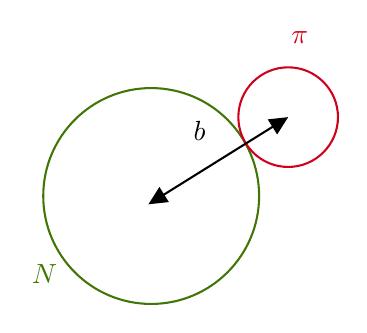
\begin{tikzpicture}[x=0.75pt,y=0.75pt,yscale=-1,xscale=1]
%uncomment if require: \path (0,300); %set diagram left start at 0, and has height of 300

%Shape: Circle [id:dp5217046923283729] 
\draw  [color={rgb, 255:red, 65; green, 117; blue, 5 }  ,draw opacity=1 ] (177,163) .. controls (177,134.28) and (200.28,111) .. (229,111) .. controls (257.72,111) and (281,134.28) .. (281,163) .. controls (281,191.72) and (257.72,215) .. (229,215) .. controls (200.28,215) and (177,191.72) .. (177,163) -- cycle ;
%Shape: Circle [id:dp22288734190325] 
\draw  [color={rgb, 255:red, 208; green, 2; blue, 27 }  ,draw opacity=1 ] (271,125) .. controls (271,111.75) and (281.75,101) .. (295,101) .. controls (308.25,101) and (319,111.75) .. (319,125) .. controls (319,138.25) and (308.25,149) .. (295,149) .. controls (281.75,149) and (271,138.25) .. (271,125) -- cycle ;
%Straight Lines [id:da9107173582949104] 
\draw    (230.21,165.41) -- (292.45,126.59) ;
\draw [shift={(295,125)}, rotate = 148.05] [fill={rgb, 255:red, 0; green, 0; blue, 0 }  ][line width=0.08]  [draw opacity=0] (8.93,-4.29) -- (0,0) -- (8.93,4.29) -- cycle    ;
\draw [shift={(227.67,167)}, rotate = 328.05] [fill={rgb, 255:red, 0; green, 0; blue, 0 }  ][line width=0.08]  [draw opacity=0] (8.93,-4.29) -- (0,0) -- (8.93,4.29) -- cycle    ;

% Text Node
\draw (170,194.4) node [anchor=north west][inner sep=0.75pt]  [color={rgb, 255:red, 65; green, 117; blue, 5 }  ,opacity=1 ]  {$N$};
% Text Node
\draw (295,82.4) node [anchor=north west][inner sep=0.75pt]  [color={rgb, 255:red, 208; green, 2; blue, 27 }  ,opacity=1 ]  {$\pi$};
% Text Node
\draw (248,125.4) node [anchor=north west][inner sep=0.75pt]  [color={rgb, 255:red, 0; green, 0; blue, 0 }  ,opacity=1 ]  {$b$};


\end{tikzpicture}
\caption{Schematic figure of the system to describe the form factor, \eqref{formfactoreq}. The pion is assumed to sit on the surface.}
\label{formfactor}
\end{marginfigure}
\begin{equation}
    \ket{p} = \mqty[1 \\ 0].
\end{equation}
From \eqref{pnpi}

\begin{equation} \label{wavefunc}
    \Psi = \mqty[\psi_p \\ \psi_{N\pi}],
\end{equation}
To construct a Hamiltonian we define two operators corresponding to creation and annihilation of the meson. We define the operator as 
\begin{marginfigure}
\centering
\tikzset{every picture/.style={line width=0.75pt}} %set default line width to 0.75pt        

\begin{tikzpicture}[x=0.75pt,y=0.75pt,yscale=-0.75,xscale=0.75]
%uncomment if require: \path (0,414); %set diagram left start at 0, and has height of 414

%Straight Lines [id:da3197661690361302] 
\draw    (150,60) -- (337.33,113.33) ;
%Straight Lines [id:da09724210631479624] 
\draw    (218.97,82.82) -- (180,190) ;
\draw [shift={(220,80)}, rotate = 109.98] [fill={rgb, 255:red, 0; green, 0; blue, 0 }  ][line width=0.08]  [draw opacity=0] (8.93,-4.29) -- (0,0) -- (8.93,4.29) -- cycle    ;

% Text Node
\draw (137,42.4) node [anchor=north west][inner sep=0.75pt]    {$N$};
% Text Node
\draw (346,112.4) node [anchor=north west][inner sep=0.75pt]    {$\pi $};
% Text Node
\draw (171,142.4) node [anchor=north west][inner sep=0.75pt]    {$\vec{R}$};
% Text Node
\draw (267,70.4) node [anchor=north west][inner sep=0.75pt]    {$\vec{r}$};
\end{tikzpicture}
\caption{Absolute and relative distance.}
\label{relativecoordinate}
\end{marginfigure}
\begin{equation} \label{W}
    W \equiv (\vec{\tau\cdot\vec{\pi}})(\vec{\sigma}\cdot\vec{r})f(r),
\end{equation}
where $f(r)$ is some form factor given by
\begin{equation}\label{formfactoreq}
    f(r) = \frac{S}{b} \text{e}^{-r^2/b^2},
\end{equation}
where $S\simeq 10 \, \text{MeV}$  and $b\simeq 1 \, \text{fm}$. This is illustrated in figure \ref{formfactor}. Note that \eqref{formfactoreq} must have units of energy per length such that \eqref{W} has units of energy. 

From \eqref{W} we can construct the Hamiltonian of the system
\begin{equation}
    H \doteq \mqty[K_{\vec{R}} & W^\dagger \\ W & K_{\vec{R}}+K_{\vec{r}}+m_\pi c^2],
\end{equation}
where $K_i$ represents the kinetic term of particle $i$. Also, $R$ represents the absolute distance and $r$ is the relative distance as illustrated in figure \ref{relativecoordinate}. Plugging this into the Schrödinger equation yields 
\begin{equation}\label{SE}
    \mqty[K_{\vec{p}} & W^\dagger \\ W & K_{\vec{R}}+K_{\vec{r}}+m_\pi c^2]\mqty[\psi_p \\ \psi_{N\pi}] = E \mqty[\psi_p \\ \psi_{N\pi}].
\end{equation}
Expanding \eqref{SE} yields two equations
\begin{align}
    K_{\vec{p}}\psi_p + W^\dagger \psi_{N\pi} = E\psi_p \label{SE1} \\
    W\psi_p + (K_{\vec{R}}+K_{\vec{r}}+m_\pi)\psi_{N\pi} = E\psi_{N\pi} \label{SE2}.
\end{align}
The first term in \eqref{SE1} vanishes and inserting \eqref{W} yields
\begin{equation}
    \int_V \text{d}^3r \, (\vec{\tau\cdot\vec{\pi}})^\dagger(\vec{\sigma}\cdot\vec{r})^\dagger f(r)\phi(r)(\vec{\tau\cdot\vec{\pi}})(\vec{\sigma}\cdot\vec{r})p\frac{1}{\sqrt{V}} = E p\frac{1}{\sqrt{V}}
\end{equation}
This can be further simplified using relations for the matrix vectors\footnote{$(\vec{\tau}\cdot \vec{\pi})^\dagger(\vec{\tau}\cdot \vec{\pi}) = 3$ \\ and
$(\vec{\sigma}\cdot \vec{r})^\dagger(\vec{\sigma}\cdot \vec{r}) = r^2$}
\begin{equation} \label{SE11}
    12\pi \int_0^\infty  \text{d}r \, f(r) \phi(r) r^4  = E.
\end{equation}
Similarly for \eqref{SE2} where the term $K_{\vec{R}}\psi_{N\pi}$ vanishes,
\begin{equation} \label{SE22}
    (\vec{\tau\cdot\vec{\pi}})(\vec{\sigma}\cdot\vec{r})f(r) p \frac{1}{\sqrt{V}}-\frac{\hbar^2}{2\mu} \nabla^2_{\vec{r}}(\vec{\tau\cdot\vec{\pi}})(\vec{\sigma}\cdot\vec{r}) p \frac{1}{\sqrt{V}}\phi(r) = (E-m_\pi c^2) (\vec{\tau\cdot\vec{\pi}})(\vec{\sigma}\cdot\vec{r}) \phi(r)p\frac{1}{\sqrt{V}},
\end{equation}
where $\mu$ is the reduced mass of the system. This equation can be further simplified by using a vector operator relation\footnote{$\nabla^2(\vec{r}\phi(r))=\vec{r}\big(\frac{\text{d}^2\phi(r)}{\text{d}r^2}+\frac{4}{r}\frac{\text{d}\phi(r)}{\text{d}r}\big)$}
\begin{equation} \label{SE23}
    f(r) -\frac{\hbar^2}{2\mu}\Big(\frac{\text{d}^2 \phi(r)}{\text{d}r^2}+\frac{4}{r}\frac{\text{d}\phi(r)}{\text{d}r}\Big) = (E-m_\pi c^2)\phi(r).
\end{equation}
This means equation \eqref{SE11} and \eqref{SE23} are the two equations that must be solved numerically.
\begin{equation} \label{system}
 \left.
    \begin{array}{ll}
            12\pi \int_0^\infty  \text{d}r \, f(r) \phi(r) r^4  = E \\
            f(r) -\frac{\hbar^2}{2\mu}\Big(\frac{\text{d}^2 \phi(r)}{\text{d}r^2}+\frac{4}{r}\frac{\text{d}\phi(r)}{\text{d}r}\Big)+m_\pi c^2 \phi(r) = E\phi(r)
    \end{array}
\right \} 
\end{equation}
\subsection{Numerical considerations}
To solve the system of equations \eqref{system} one can consider two different numerical approaches. 

For a given $E$ one can solve the second order corresponding to $\phi[E]$. Conversely, for a given $\phi(r)$ one can calculate the integral to find $E[\phi]$. This leads to the fixed-point equation given by
\begin{equation} \label{nonlin}
    E[\phi[\mathcal{E}]] = \mathcal{E},
\end{equation}
which is a single variable non-linear equation. \eqref{nonlin} can be solved using a root-finding algorithm.

The second approach consists of reformulating the system \eqref{system} as a boundary value problem with the following conditions
\begin{equation}
    I'(r) = 12\pi f(r)\phi(r)r^4, \quad I(0)=0, \, I(\infty)=E.
\end{equation}
The equation starts from a singular point and extends to an infinite point. Considerations about how to scale the starting point and stopping point as a function of $b$ are needed. These two points must be proportional to $b$ with some arbitrary proportionality constant. In the regime of nuclear physics we expect the wavefunction to extend up to a length within the order of magnitude of ten Fermi. 

We require the solution to stay finite which means approximations are needed at both limits. At $r\rightarrow 0$ the differential equation is approximately an Euler-Cauchy equation with basis solutions $1$ and $r^{-1}$. For finite solutions the latter is ignored which means $\phi'(a)=0$ is the requirement for $a\approx 0$.\footnote{You would end up with the same conclusion if you consider $\phi=a+r^n$ and plug this into $\phi''+4\phi'/r=0$, which yields $n=0,-1$.} For $r\rightarrow \infty$ the dominating term is the differential equation are
\begin{equation}
    -\phi''(r)+2\mu(m_\pi c^2-E)\phi(r)=0.
\end{equation}
Since we expect a negative value for $E$ the basis solutions are \\ $\exp{\pm\sqrt{2\mu(m_\pi c^2+\abs{E})}}r$. In the case of a positive sign the solution diverges. For the basis solution with negative exponents we have
\begin{equation}
    \phi'(r)+\sqrt{2\mu(m_\pi c^2 +\abs{E})}\phi(r)=0.
\end{equation}
These two conditions are suitable boundary conditions for the left and right boundaries, respectively. The solutions can be seen in figure \ref{fig:integralplot}.
\begin{figure}[H]
    \begin{sidecaption}{Boundary value problem solutions. The plot is generated using a tolerance of $10^{-6}$. The RMS values of the relative residuals over each mesh intervals is shown in the Appendix. For clarity, I have scaled the energy.}[fig:integralplot]
    \includegraphics[width=\linewidth]{Figures/Integralplot.pdf}
    \end{sidecaption}
\end{figure}
The algorithm converges and a solution to \eqref{SE} is found. Also, note that since we expect the energy to be less than zero it makes sense for the wavefunction to be negative since all other terms in the integral are positive. This also makes sense since we are adding more degrees of freedom to the system, which means the energy in turn must decrease. In figure \ref{fig:integralplot} I have scaled the energy for plotting aesthetics. The actual energy is given by
\begin{equation}
E = -0.626 \, \text{MeV}.
\end{equation}
This energy will act as a zero-point energy in the rest of the calculations. Note that this energy is found without any considerations about the velocity of the pion below the potential barrier. Strictly speaking, some considerations about the kinematic limit of the pion is needed to more robustly confirm the energy, which is essential to the rest of the calculations.
\subsection{Relativistic Expansion}
 It is customary to assume a nonrelativistic limit when considering regular quantum mechanics. To account for relativistic effect we can replace the kinetic term, $K_{\vec{r}}$ in \eqref{SE}
 \begin{equation}
     K_{\vec{r}}\rightarrow K_{\vec{r},\text{rel}} = \sqrt{p^2 c^2+\mu^2 c^4} = \mu c^2 \bigg(\sqrt{1+\frac{p^2}{\mu^2 c^2}}-1 \bigg),
 \end{equation}
\begin{marginfigure}
\centering


\tikzset{every picture/.style={line width=0.75pt}} %set default line width to 0.75pt        

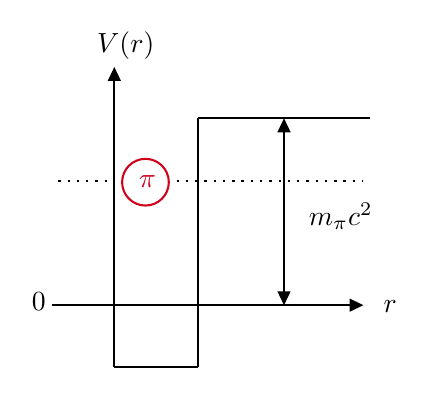
\begin{tikzpicture}[x=0.75pt,y=0.75pt,yscale=-0.75,xscale=0.75]
	%uncomment if require: \path (0,462); %set diagram left start at 0, and has height of 462
	
	%Straight Lines [id:da04487003009359902] 
	\draw    (276,240) -- (276,90) ;
	\draw [shift={(276,87)}, rotate = 90] [fill={rgb, 255:red, 0; green, 0; blue, 0 }  ][line width=0.08]  [draw opacity=0] (8.93,-4.29) -- (0,0) -- (8.93,4.29) -- cycle    ;
	%Straight Lines [id:da11984458862135328] 
	\draw    (236,240) -- (433,240) ;
	\draw [shift={(436,240)}, rotate = 180] [fill={rgb, 255:red, 0; green, 0; blue, 0 }  ][line width=0.08]  [draw opacity=0] (8.93,-4.29) -- (0,0) -- (8.93,4.29) -- cycle    ;
	%Straight Lines [id:da39644848633047847] 
	\draw    (330,280) -- (330,120) ;
	%Straight Lines [id:da23479083436400994] 
	\draw    (330,280) -- (297,280) -- (276,280) ;
	%Straight Lines [id:da22091112894519627] 
	\draw    (276,240) -- (276,280) ;
	%Straight Lines [id:da47586844464292766] 
	\draw  [dash pattern={on 0.84pt off 2.51pt}]  (240,160) -- (276,160) ;
	%Straight Lines [id:da07090607985351194] 
	\draw  [dash pattern={on 0.84pt off 2.51pt}]  (316,160) -- (436,160) ;
	%Flowchart: Connector [id:dp0772408562939938] 
	\draw  [color={rgb, 255:red, 208; green, 2; blue, 27 }  ,draw opacity=1 ] (281,161) .. controls (281,152.72) and (287.72,146) .. (296,146) .. controls (304.28,146) and (311,152.72) .. (311,161) .. controls (311,169.28) and (304.28,176) .. (296,176) .. controls (287.72,176) and (281,169.28) .. (281,161) -- cycle ;
	%Straight Lines [id:da8208549108465544] 
	\draw    (330,120) -- (440,120) ;
	%Straight Lines [id:da059140841724983684] 
	\draw    (385,237) -- (385,123) ;
	\draw [shift={(385,120)}, rotate = 90] [fill={rgb, 255:red, 0; green, 0; blue, 0 }  ][line width=0.08]  [draw opacity=0] (8.93,-4.29) -- (0,0) -- (8.93,4.29) -- cycle    ;
	\draw [shift={(385,240)}, rotate = 270] [fill={rgb, 255:red, 0; green, 0; blue, 0 }  ][line width=0.08]  [draw opacity=0] (8.93,-4.29) -- (0,0) -- (8.93,4.29) -- cycle    ;
	
	% Text Node
	\draw (263,62.4) node [anchor=north west][inner sep=0.75pt]    {$V(r)$};
	% Text Node
	\draw (447,235) node [anchor=north west][inner sep=0.75pt]    {$r$};
	% Text Node
	\draw (290,155) node [anchor=north west][inner sep=0.75pt]  [color={rgb, 255:red, 208; green, 2; blue, 27 }  ,opacity=1 ]  {$\pi $};
	% Text Node
	\draw (221,230) node [anchor=north west][inner sep=0.75pt]    {$0$};
	% Text Node
	\draw (399,172.4) node [anchor=north west][inner sep=0.75pt]    {$m_{\pi } c^{2}$};
	
	
\end{tikzpicture}
\caption{Illustration of the pion under the barrier. We are considering the kinetic expansion of the pion in this regime. The behavior of the potential barrier is a sketch.}
\label{fig:UnderBarrier}
\end{marginfigure}  
 where $\mu$ is the reduces mass of the nucleon-pion system. This leads to a new systems of equations and these solutions can be compared found in the nonrelativistic limit to deduce with relativistic regime dominates the physical setup. More specifically we can compare the energy ratios denoted by $E_R$. Starting from \eqref{SE2}
 \begin{equation}
     f(r) (\vec{\tau} \cdot \vec{\pi})(\vec{\sigma}\cdot \vec{r})\psi_p + \mu c^2 \bigg(\sqrt{1+\frac{p^2}{\mu^2 c^2}}-1 \bigg)\psi_{N\pi} = (E-m_{\pi}c^2)\psi_{N\pi},
 \end{equation}
 This equation turns out to be divergent and we must therefor resort to an approximation. The kinetic energy is expanded
 \begin{equation}
     K_{\vec{r},\text{rel}} = \mu c^2\sqrt{1+\frac{p^2}{\mu^2}}-\mu c^2 \approx \frac{p^2}{2\mu}-\frac{p^4}{8\mu^3 c^2}
 \end{equation}
 This means we get an extra term in \eqref{SE22} yielding
 \begin{equation}
     f(r)\vec{r}-\bigg( \frac{p^2}{2\mu}-\frac{p^4}{8\mu^3 c^3} \bigg)\vec{r}\phi(r) = (E-m_\pi c^2)\vec{r}\phi(r)
 \end{equation}
 Using the vector operators yields the following expression\footnote{\begin{align*}
     \nabla^4(\vec{r}\phi(r))&=\nabla^2(r\phi''+4\phi') \\
     &= 2\phi''''+2(\nabla\phi''\cdot\nabla)r+4\phi''') \\
     &=r\phi''''+6\phi'''
 \end{align*}}
 \begin{equation}
    f(r)-\frac{\hbar^2}{2\mu}\bigg( \phi^{(2)}(r)+\frac{4}{r}\phi^{(1)}(r) \bigg)+\frac{\hbar^3}{8\mu^3 c^3}\bigg(\phi^{(4)}(r)+\frac{6}{r}\phi^{(3)}(r)\bigg)=(E-m_\pi c^2)\phi(r),
 \end{equation}
 where the exponent, $(n)$, is the order the differentiation. This leads to a system of equations given by
 \begin{equation} \label{systemrel}
 \left.
    \begin{array}{ll}
            12\pi \int_0^\infty  \text{d}r \, f(r) \phi(r) r^4  = E \\
               f(r)-\frac{\hbar^2}{2\mu}\big( \phi^{(2)}(r)+\frac{4}{r}\phi^{(1)}(r) \big)+\frac{\hbar^4}{8\mu^3 c^3}\big(\phi^{(4)}(r)+\frac{6}{r}\phi^{(3)}(r)\big)=(E-m_\pi c^2)\phi(r)
    \end{array}
\right \} 
\end{equation}
This system is a fourth order differential equation coupled to an integrodifferential equation and is solved using the boundary value problem technique. The boundary conditions can be found using the same considerations as in the previous section. For $r\rightarrow \infty$ the dominating terms are 
\begin{equation}
    \phi^{(4)}(r) = 8\mu^3(E-m_\pi c^2) \phi^{(1)}(r)+4\mu \phi^{(2)}(r)
\end{equation}
The solutions are shown in figure \ref{fig:integralplot_relativistic}
\begin{figure}[H]
    \begin{sidecaption}{Boundary value problem solutions for the relativistic expansion. The plot is generated using a tolerance of $10^{-3}$. The energy convergence is scaled.}[fig:integralplot_relativistic]
    \includegraphics[width=\linewidth]{Figures/Integralplot_relativistic.pdf}
    \end{sidecaption}
\end{figure}
Let me show a plot for yall
\begin{figure}[H]
    \begin{sidecaption}{Plots for different values of the parameters $S$ and $b$ to illustrate the difference between the nonrelativistic equations and the relativistic equations. }[fig:relativistic_expansion]
    \includegraphics[width=\linewidth]{Figures/RelativisticExpansion.pdf}
    \end{sidecaption}
\end{figure}
From figure \ref{fig:relativistic_expansion} one can also deduce the effect of changing the parameters $S,b$ corresponding to changing the physical coupling strength and the form factor. Increasing the parameter $b$ will flatten the wavefunction which will decrease the energy. This corresponds to increasing the distance between the pion and the nucleus. Increasing the coupling strength $S$ will increase the amplitude of the wave function.
\section{Pion photoproduction}\label{sec:dipoleapprox}
We now consider the case of pion photoproduction. We consider an initial (bound) state given by
\begin{equation} \label{phii}
    \ket{\Phi_i} = \mqty[\phi_p \\ \phi_{N\pi}],
\end{equation}
where $\phi$ represents a bound state. The final state consists of the same superposition but in an unbound system represented by $\psi$, i.e.
\begin{equation} \label{psif}
    \ket{\Psi_f} = \mqty[\psi_p \\ \psi_{N\pi}].
\end{equation}
\subsection{Normalization of the initial state}\label{subsec:initial}
We must also impose some normalization. Starting from \eqref{phii}
\begin{align}
    \Phi = \mathcal{N} \mqty[p\uparrow \\ (\vec{\tau}\cdot \vec{\pi})(\vec{\sigma}\cdot \vec{r})p\uparrow \phi(r)],
\end{align}
where $\uparrow$ represents the spin state, $\phi(r)$ is the wavefunction from figure  \ref{fig:integralplot} and $\mathcal{N}$ is the normalization constant.
This leads to
\begin{align}
    \braket{\Phi}{\Phi} &= \abs{\mathcal{N}}^2 \big( \braket{\phi_p}{\phi_p}+ \braket{\phi_{N\pi}}{\phi_{N\pi}} \big) \\
    &= \abs{\mathcal{N}}^2 \big( V+3V\int \text{d}^3r \, r^2 \phi(r)^2 \big)\label{int} \\
    &\stackrel{!}{=} 1.
\end{align} 
This leads to the following normalization constant
\begin{equation}
    \mathcal{N} = \frac{1}{\sqrt{V}}\frac{1}{\sqrt{1+\epsilon}},
\end{equation}
where $V$ is the volume and $\epsilon$ is the integral in \eqref{int}. To figure out what particle can be knocked out by a photon via photodisintegration we consider the pion channel in \eqref{psif}. 
This expression is the properly normalized initial state.
\subsection{Normalization of the final state}\label{subsec:final}
The final state consists of the unbound system represented by $\psi$. Expanding the terms using the isospin operators yields\footnote{$\tau_0 \pi^0 + \sqrt{2}\tau_+\pi^-+\sqrt{2}\tau_-\pi^+$}
\begin{equation} \label{phiinitial}
    \phi_{N\pi} = c(\vec{\tau}\cdot \vec{\pi})(\vec{\sigma}\cdot \vec{r})p\uparrow \phi(r) = c(p\pi^0+\sqrt{2}n\pi^+)(\vec{\sigma}\cdot \vec{r})\uparrow \phi(r).
\end{equation}
From this equation the first result should be highlighted. We consider two photodisintegration processes
\begin{align}
     p\gamma & \rightarrow p\pi^0 \\
     p\gamma & \rightarrow n \pi^+,
\end{align}
where due to orthogonality of the states in isospin space the process involves the neutron is proportional to $\sqrt{2}$. Since this term will exist throughout the calculations we know the ratio between these two processes must be related by a factor of 2. There are also some corrections related to the mass difference between the proton and the neutron. This will be evident when comparing the matrix elements in section \ref{sec:dipoles}. By expanding the matrices in spin space and using the spherical tensor operator we see
\begin{equation}\label{spinmatrix}
    (\vec{\sigma}\cdot \vec{r}) = \sqrt{\frac{4\pi}{3}} r \mqty[Y_{1}^0 & \sqrt{2}Y_1^{-1} \\ \sqrt{2}Y_1^1 & Y_1^0],
\end{equation}
\begin{marginfigure}
\centering


\tikzset{every picture/.style={line width=0.75pt}} %set default line width to 0.75pt        

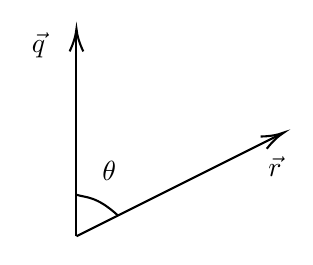
\begin{tikzpicture}[x=0.75pt,y=0.75pt,yscale=-1,xscale=1]
%uncomment if require: \path (0,300); %set diagram left start at 0, and has height of 300

%Straight Lines [id:da4402999370947803] 
\draw    (250,150) -- (250,52) ;
\draw [shift={(250,50)}, rotate = 90] [color={rgb, 255:red, 0; green, 0; blue, 0 }  ][line width=0.75]    (10.93,-3.29) .. controls (6.95,-1.4) and (3.31,-0.3) .. (0,0) .. controls (3.31,0.3) and (6.95,1.4) .. (10.93,3.29)   ;
%Straight Lines [id:da0037929251539179365] 
\draw    (250,150) -- (348.21,100.89) ;
\draw [shift={(350,100)}, rotate = 153.43] [color={rgb, 255:red, 0; green, 0; blue, 0 }  ][line width=0.75]    (10.93,-3.29) .. controls (6.95,-1.4) and (3.31,-0.3) .. (0,0) .. controls (3.31,0.3) and (6.95,1.4) .. (10.93,3.29)   ;
%Curve Lines [id:da06140636400336408] 
\draw    (250,130) .. controls (254.53,131.45) and (259.53,130.45) .. (270,140) ;

% Text Node
\draw (227,50.4) node [anchor=north west][inner sep=0.75pt]    {$\vec{q}$};
% Text Node
\draw (341,110.4) node [anchor=north west][inner sep=0.75pt]    {$\vec{r}$};
% Text Node
\draw (261,112.4) node [anchor=north west][inner sep=0.75pt]    {$\theta $};


\end{tikzpicture}
\caption{Illustration of the angle between the two vectors $\vec{q}$ and $\vec{r}$ in equation (\ref{expansion})}
\label{normsphere}
\end{marginfigure}
where, similar to in isospin space, the off-diagonals include a factor $\sqrt{2}$. This expansion will be useful when evaluating matrix elements with the different spin states represented by $(\uparrow \downarrow)$. Considering the final state which consists of a plane wave. It is useful to expand this in terms of spherical harmonics. Using the spherical harmonic decomposition of the plane wave yields

\begin{align}
    \frac{1}{\sqrt{V}} \text{e}^{-i\vec{q}\cdot\vec{r}} &= \frac{1}{\sqrt{V}} \sum_{\ell,m} 4\pi i^\ell Y_\ell^{*m}(\vec{q})Y_\ell^m(\vec{r})j_\ell(qr) \\
    &= \frac{1}{\sqrt{V}} \sum_\ell 4\pi i^\ell j_\ell(qr) \bigg( \frac{2\ell+1}{4\pi}\bigg)P_\ell(\cos\theta),
\end{align}
where $\theta$ is the angle between $\vec{q}$ and $\vec{r}$ also illustrated on \ref{normsphere} and $P_\ell$ is the Legendre polynomial of degree $\ell$. For now $\vec{q}$ is some variable related to the energy of the photon and will act as momentum. This is illustrated on figure \ref{fig:qenergy} and is expanded upon in the next section. Also, the spherical harmonic addition theorem has been used.\footnote{$\sum_m Y_\ell^m(\vec{p}')Y_\ell^{*m}(\vec{r})=\big( \frac{2\ell+1}{4\pi}\big)P_\ell(\cos\theta)$} Since we are considering the pion channnel just above the threshold we do the following expansion
\begin{equation} \label{expansion}
\frac{1}{\sqrt{V}}\text{e}^{i\vec{q}\cdot \vec{r}} \stackrel{\ell=0}{=} \frac{1}{\sqrt{V}}j_0(qr),    
\end{equation}
which is assumed to be the dominant contribution
\subsection{Photoproduction: dipole approximation}\label{sec:dipoles}
We now move on to the actual matrix element we want to calculate 
\begin{equation}
    \mel{\Psi_f}{\vec{d}}{\Phi_i},
\end{equation}
where $\vec{d}$ is the dipole operator, $\ket{\Phi_i}$ and $\ket{\Psi_f}$ are given by \eqref{phii} and \eqref{psif} respectively. As before, we only consider the pion channel. Since we are considering transitions just above the threshold we only consider the contributions from the electric dipole term. This terms is assumed to dominate and higher order terms can be calculated later if necessary. Considering the pion channel for the following process $p \gamma \rightarrow n\pi^+$
\begin{equation}
    \mathcal{M}=-i\omega_k\sqrt{\frac{2\pi\hbar}{V\omega_{\vec{k}}}}\vec{e}_{\vec{k},\lambda}\mel*{\frac{1}{\sqrt{V}}\text{e}^{i\vec{q}\cdot \vec{r}}n\pi^+ (\uparrow \downarrow)}{\vec{d}}{(\vec{\tau}\cdot \vec{\pi})(\vec{\sigma}\cdot \vec{r})p\uparrow \phi(r)\mathcal{N}}
\end{equation}
where the two arrows represents the two spin states of the neutron and the proton. Also, $q$ is illustrated in figure \ref{fig:qenergy} where the energy, $E$, is the same as in \eqref{system}. This is the zero point energy in the system we are considering and can be written as 
\begin{marginfigure}
\centering


\tikzset{every picture/.style={line width=0.75pt}} %set default line width to 0.75pt        

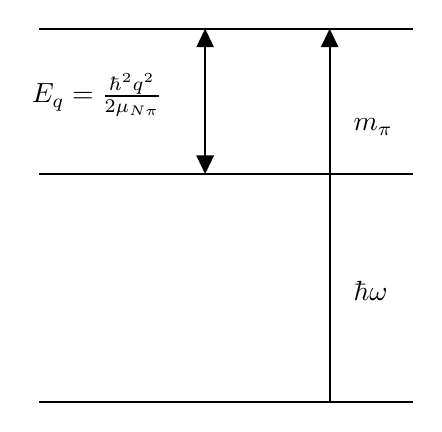
\begin{tikzpicture}[x=0.75pt,y=0.75pt,yscale=-1,xscale=1]
	%uncomment if require: \path (0,300); %set diagram left start at 0, and has height of 300
	
	%Straight Lines [id:da9050164165880492] 
	\draw    (210,200) -- (390,200) ;
	%Straight Lines [id:da595724624922532] 
	\draw    (210,90) -- (390,90) ;
	%Straight Lines [id:da8326738532712242] 
	\draw    (210,20) -- (390,20) ;
	%Straight Lines [id:da4515077860512252] 
	\draw    (350,200) -- (350,23) ;
	\draw [shift={(350,20)}, rotate = 90] [fill={rgb, 255:red, 0; green, 0; blue, 0 }  ][line width=0.08]  [draw opacity=0] (8.93,-4.29) -- (0,0) -- (8.93,4.29) -- cycle    ;
	%Straight Lines [id:da5226155750538098] 
	\draw    (290,87) -- (290,23) ;
	\draw [shift={(290,20)}, rotate = 90] [fill={rgb, 255:red, 0; green, 0; blue, 0 }  ][line width=0.08]  [draw opacity=0] (8.93,-4.29) -- (0,0) -- (8.93,4.29) -- cycle    ;
	\draw [shift={(290,90)}, rotate = 270] [fill={rgb, 255:red, 0; green, 0; blue, 0 }  ][line width=0.08]  [draw opacity=0] (8.93,-4.29) -- (0,0) -- (8.93,4.29) -- cycle    ;
	
	% Text Node
	\draw (360,140) node [anchor=north west][inner sep=0.75pt]    {$\hbar \omega $};
	% Text Node
	\draw (360,62) node [anchor=north west][inner sep=0.75pt]    {$m_{\pi }$};
	% Text Node
	\draw (205,40) node [anchor=north west][inner sep=0.75pt]    {$E_{q} =\frac{\hbar ^{2} q^{2}}{2\mu _{N\pi }}$};
	
	
\end{tikzpicture}
\caption{Illustration of the energy levels. Here the energy $E$ refers to the energy shown in \ref{fig:integralplot} and will act as a zero-point enery.}
\label{fig:qenergy}
\end{marginfigure}  
\begin{equation}
    \frac{\hbar^2 q^2}{2\mu_{N\pi}} = \hbar \omega-m_\pi c^2,
\end{equation}
where $\mu_{N\pi}$ is the reduced mass of the nucleon-pion system. Compare this equation to \eqref{kq}. The front factor arises from the quantization of the electromagnetic field. Using the results from section \ref{subsec:final} and section \ref{subsec:initial}. The different spin states of the neutron in the final state yields to contributions to the total matrix element given by
\begin{align}
    \mathcal{M}^{\uparrow} &=\frac{-i\mathcal{N}\sqrt{2}\omega_k\vec{e}_{\vec{k},\lambda}}{V}\sqrt{\frac{2\pi\hbar}{V\omega_{\vec{k}}}}\mel*{j_0(qr)}{d_0 r_0}{\phi(r)}  \\
    &= \frac{-i\mathcal{N}\sqrt{2}\omega_k\vec{e}_{\vec{k},\lambda}}{V}\sqrt{\frac{2\pi\hbar}{V\omega_{\vec{k}}}}\sqrt{\frac{4\pi}{3}}\mel*{j_0(qr)}{d_0 r Y_1^0}{\phi(r)} \\
    \mathcal{M}^{\downarrow} & = \frac{-i\mathcal{N}2\omega_k\vec{e}_{\vec{k},\lambda}}{V}\sqrt{\frac{2\pi\hbar}{V\omega_{\vec{k}}}} \mel{j_0(qr)}{d r_{+}}{\phi(r)}\\
    &=\frac{-i\mathcal{N}2\omega_k\vec{e}_{\vec{k},\lambda}}{V}\sqrt{\frac{2\pi\hbar}{V\omega_{\vec{k}}}}\sqrt{\frac{4\pi}{3}}\mel*{j_0(qr)}{d_0 r Y_1^1}{\phi(r)}, \\
\end{align}
where the spin down state picks up a factor $\sqrt{2}$ from equation \ref{spinmatrix}. Now we calculate the remaining matrix elements,
\begin{align}
    \mel{j_0(qr)}{d_0 r_0}{\phi(r)} &= \frac{\mu}{m_\pi}e \mel{j_0(qr)}{r_0r_0}{\phi(r)} \\
    &= \frac{\mu}{m_\pi}e\frac{4\pi}{3} \mel{j_0}{r^2}{\phi(r)} \\
    &= \frac{\mu e }{m_\pi} \int_0^\pi \int_0^{2\pi} \int_0^\infty \text{d}r \text{d}\phi \text{d}\theta \, j_0(qr)r^4\cos^2\theta \sin\theta \phi(r) \\
    &= \frac{4\pi \mu e}{3m_\pi} \underbrace{\int_0^\infty \text{d}r \, j_0(qr)r^4\phi(r)}_{\mathcal{Q}},
\end{align}
where the dipole operator has been inserted and the angular integrals calculated. Similarly for the next matrix element,
\begin{align}
    \mel{j_0(qr)}{d_{-}r_{+}}{\phi(r)} &= \frac{\mu}{m_\pi}e \mel{j_0(qr)}{r_{-}r_{+}}{\phi(r)} \\
    &= \frac{4\pi \mu e}{3 m_\pi} \mel{j_0(qr)}{r^2 Y_1^{-1}Y_1^1}{\phi(r)} \\
    &= \frac{4\pi \mu e}{3 m_\pi} \mathcal{Q}. 
\end{align}
This leads to the two final expressions for the two matrix elements
\begin{equation}
    \abs{\mathcal{M}^\uparrow} = \bigg( \frac{4\pi \mu e}{3m_\pi}\bigg)^2 \frac{2 \mathcal{N}^2\omega_k (2\pi \hbar)}{V^2}(\vec{e}_{\vec{k},\lambda})^0(\vec{e}_{\vec{k},\lambda}^*)^0 \mathcal{Q}^2 
\end{equation}
Similarly for the next matrix element
\begin{equation}
    \abs{\mathcal{M}^\downarrow} = \bigg( \frac{4\pi \mu e}{3 m_\pi}\bigg)^2 \frac{4\mathcal{N}\omega_{\vec{k}}(2\pi\hbar)}{V^2}(\vec{e}_{\vec{k},\lambda})^+(\vec{e}_{\vec{k},\lambda}^*)^+ \mathcal{Q}^2.
\end{equation}
Calculating the total matrix element using a polarization theorem\footnote{$(\vec{e}_{\vec{k},\lambda}^*\cdot \vec{e}_{\vec{k},\lambda})=\delta_{\lambda,\lambda'}$ and $\vec{e}_{\vec{k},\mp}=\pm\frac{1}{\sqrt{2}}(\vec{e}_{\vec{k},1}\pm i\vec{e}_{\vec{k},2})$. This leads to $(\vec{e}^{0*}_{\vec{k},\lambda}\cdot\vec{e}^{0}_{\vec{k},\lambda'})+(\vec{e}^{0+}_{\vec{k},\lambda}\cdot\vec{e}^{+}_{\vec{k},\lambda'})=\delta_{\lambda,\lambda'}+\frac{1}{2}\delta_{\lambda,\lambda'}$}
\begin{align}
    \abs{\mathcal{M}}^2 &= \abs{\mathcal{M}^\uparrow}^2 + \abs{\mathcal{M}^\downarrow}^2 \\
    &= \frac{2\pi \hbar \omega_k \mathcal{N}^2 e^2}{V^2} \bigg( \frac{4\pi\mu}{3m_\pi}\bigg)^2 \mathcal{Q}^2,
\end{align}
which is the final expression for the matrix element. According to Fermi's golden rule we can calculate the transition probability
\begin{equation}\label{domega}
    \text{d}\omega = \frac{2\pi}{\hbar} \abs{\mathcal{M}}^2 \text{d}\rho,
\end{equation}
where the density of states is given by
\begin{equation}\label{densityofstates}
    \text{d}\rho = \frac{Vqm }{\hbar^2 (2\pi)^3}\text{d}\Omega.
\end{equation}
This is related to the differential cross section 
\begin{equation}\label{diffcrosssection}
    \frac{\text{d}\sigma}{\text{d}\Omega}=\frac{16 \pi}{9} \mathcal{N}^2 \alpha \bigg(\frac{\mu}{m_\pi} \bigg)^2 \frac{\omega_k q\mu}{\hbar^2}\mathcal{Q}^2
\end{equation}
This should be compared to experimental data shown in figure \ref{fig:pgammacross}
\begin{figure}[H]
    \begin{sidecaption}{Experimental total cross section for $\gamma p$. Data from}[fig:pgammacross]
    \includegraphics[width=\linewidth]{Figures/pgammaexperiment.pdf}
    \end{sidecaption}
\end{figure}
\section{Pion Photoproduction exact}
In section \ref{sec:dipoleapprox} we looked at how to use the model described in section \ref{sec:model} to get an expression for the cross section which was compared to experimental data. More specifically we used the dipole approximation which introduces a trade-off between the difficulty of the calculations and the regime in which our solution is valid. We expect the dipole approximation to hold for low energies just above the threshold. To both validate and generalize this result we now do a different approach and calculate the cross section exact and also consider recoil effects. Strictly speaking, recoil effects should also be considered in section \ref{sec:dipoleapprox} since the mass ratio between the nucleon and the pion cannot be assumed to yield a stationary nucleon after the pion photoproduction process. To calculate the exact matrix elements we consider a non-relativistic system of particles interacting with the electromagnetic field. The interacting part of the Hamiltonian is given by
\begin{equation} \label{firstinthamil}
	H = \frac{1}{2m_\pi} \bigg( \vec{p}-\frac{e}{c}\vec{A}(\vec{r}) \bigg)^2,
\end{equation}
where $\vec{p}$ is the momentum operator and $\vec{A}(\vec{r})$ is the quantized vector potential at the point $\vec{r}$. Note that we have already replaced the usual mass by the mass of the pion, $m_\pi$ since we are considering the interaction of a pion with charge $e$ with the electromagnetic field. 

The electromagnetic interaction is relatively weak compared to the strong force. For our problem, this means we can expand the interaction by taking only the lowest non-vanishing order of perturbation into account. Since we later want to consider transition probabilities we only keep the first non-linear term of \eqref{firstinthamil} which yields
\begin{equation}\label{secondinthamil}
	V^{(1)} = -\frac{e}{2m_\pi c}\bigg( \vec{p}\cdot \vec{A}(\vec{r}_\pi,t)+\vec{A}(\vec{r}_\pi,t)\cdot \vec{p}\bigg),
\end{equation}
\begin{marginfigure}
	\centering
	

\tikzset{every picture/.style={line width=0.75pt}} %set default line width to 0.75pt        

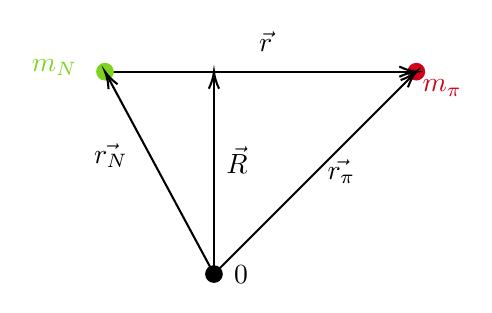
\begin{tikzpicture}[x=0.75pt,y=0.75pt,yscale=-0.75,xscale=0.75]
	%uncomment if require: \path (0,300); %set diagram left start at 0, and has height of 300
	
	%Flowchart: Connector [id:dp9827455772611288] 
	\draw  [color={rgb, 255:red, 208; green, 2; blue, 27 }  ,draw opacity=1 ][fill={rgb, 255:red, 208; green, 2; blue, 27 }  ,fill opacity=1 ] (315,90) .. controls (315,87.24) and (317.24,85) .. (320,85) .. controls (322.76,85) and (325,87.24) .. (325,90) .. controls (325,92.76) and (322.76,95) .. (320,95) .. controls (317.24,95) and (315,92.76) .. (315,90) -- cycle ;
	%Straight Lines [id:da5093684133345362] 
	\draw    (125,90) -- (318,90) ;
	\draw [shift={(320,90)}, rotate = 180] [color={rgb, 255:red, 0; green, 0; blue, 0 }  ][line width=0.75]    (10.93,-3.29) .. controls (6.95,-1.4) and (3.31,-0.3) .. (0,0) .. controls (3.31,0.3) and (6.95,1.4) .. (10.93,3.29)   ;
	%Straight Lines [id:da04984112064582158] 
	\draw    (190,220) -- (190,92) ;
	\draw [shift={(190,90)}, rotate = 90] [color={rgb, 255:red, 0; green, 0; blue, 0 }  ][line width=0.75]    (10.93,-3.29) .. controls (6.95,-1.4) and (3.31,-0.3) .. (0,0) .. controls (3.31,0.3) and (6.95,1.4) .. (10.93,3.29)   ;
	%Straight Lines [id:da13661676787341415] 
	\draw    (190,220) -- (318.59,91.41) ;
	\draw [shift={(320,90)}, rotate = 135] [color={rgb, 255:red, 0; green, 0; blue, 0 }  ][line width=0.75]    (10.93,-3.29) .. controls (6.95,-1.4) and (3.31,-0.3) .. (0,0) .. controls (3.31,0.3) and (6.95,1.4) .. (10.93,3.29)   ;
	%Flowchart: Connector [id:dp37210275318157304] 
	\draw  [color={rgb, 255:red, 126; green, 211; blue, 33 }  ,draw opacity=1 ][fill={rgb, 255:red, 126; green, 211; blue, 33 }  ,fill opacity=1 ] (115,90) .. controls (115,87.24) and (117.24,85) .. (120,85) .. controls (122.76,85) and (125,87.24) .. (125,90) .. controls (125,92.76) and (122.76,95) .. (120,95) .. controls (117.24,95) and (115,92.76) .. (115,90) -- cycle ;
	%Straight Lines [id:da8769015497622031] 
	\draw    (190,220) -- (120.95,91.76) ;
	\draw [shift={(120,90)}, rotate = 61.7] [color={rgb, 255:red, 0; green, 0; blue, 0 }  ][line width=0.75]    (10.93,-3.29) .. controls (6.95,-1.4) and (3.31,-0.3) .. (0,0) .. controls (3.31,0.3) and (6.95,1.4) .. (10.93,3.29)   ;
	%Flowchart: Connector [id:dp5562170943538245] 
	\draw  [color={rgb, 255:red, 0; green, 0; blue, 0 }  ,draw opacity=1 ][fill={rgb, 255:red, 0; green, 0; blue, 0 }  ,fill opacity=1 ] (185,220) .. controls (185,217.24) and (187.24,215) .. (190,215) .. controls (192.76,215) and (195,217.24) .. (195,220) .. controls (195,222.76) and (192.76,225) .. (190,225) .. controls (187.24,225) and (185,222.76) .. (185,220) -- cycle ;
	
	% Text Node
	\draw (71,80.4) node [anchor=north west][inner sep=0.75pt]  [color={rgb, 255:red, 126; green, 211; blue, 33 }  ,opacity=1 ]  {$m_{N}$};
	% Text Node
	\draw (322,93.4) node [anchor=north west][inner sep=0.75pt]  [color={rgb, 255:red, 208; green, 2; blue, 27 }  ,opacity=1 ]  {$m_{\pi }$};
	% Text Node
	\draw (196,136.4) node [anchor=north west][inner sep=0.75pt]    {$\vec{R}$};
	% Text Node
	\draw (261,144.4) node [anchor=north west][inner sep=0.75pt]    {$\vec{r_{\pi }}$};
	% Text Node
	\draw (111,134.4) node [anchor=north west][inner sep=0.75pt]    {$\vec{r_{N}}$};
	% Text Node
	\draw (217,62.4) node [anchor=north west][inner sep=0.75pt]    {$\vec{r}$};
	% Text Node
	\draw (201,212.4) node [anchor=north west][inner sep=0.75pt]    {$0$};
	
	
\end{tikzpicture}
	\caption{Jacobi coordinates illustrating $\vec{r}_\pi$ used in the vector potential in equation \ref{thirdinthamil}. Here we use $\vec{r}=\vec{r}_\pi-\vec{r}_N$ and see that $\vec{r}_\pi = \vec{R}+\vec{r}\frac{m_N}{M}$, where $M=m_N+m_\pi$.}
	\label{JacobiIllustration}
\end{marginfigure}
\noindent which also means the interacting part is linear in the creation(annihilation) operators corresponding to single-photon emission(absorption). Our choice of gauge is purely conventional and we choose the radiation gauge which imposes a condition on the vector potential given by
\begin{equation}
	\nabla \cdot \vec{A} = 0,
\end{equation}
and this is a convenient choice of gauge since the commutator in \eqref{secondinthamil} is $\nabla \cdot \vec{A}$ and we can write
\begin{equation}\label{thirdinthamil}
	V^{(1)} = -\frac{e}{m_\pi c}\vec{A}(\vec{r_\pi},t)\cdot \vec{p}_\pi. 
\end{equation}
Note that \eqref{thirdinthamil} consists of the pion momentum operator, $\vec{p}_\pi$ and the electromagnetic vector potential at a distance $r_\pi$. This distance was also mentioned in section \ref{sec:model} and can be expressed in term of the Jacobi coordinates illustrated on figure \ref{JacobiIllustration} where the relative coordinate is given by $\vec{r}=\vec{r}_\pi-\vec{r}_N$ which leads to the following transformation of equation \eqref{thirdinthamil}
\begin{equation}
	V^{(1)} = -\frac{e}{m_\pi c}\vec{A}(\vec{r_\pi},t)\cdot \vec{p}_\pi = \frac{-e}{m_\pi} \bigg( \vec{p}+\frac{m_N}{M}\vec{P}\bigg)\vec{A}\bigg(\vec{R}+\frac{m_N}{M}\vec{r},t\bigg),
\end{equation}
where $M=m_N+m_\pi$ is the total mass of the system. We now move on from the general theory of the pion interacting with the electromagnetic field and consider the specific case of pion photoproduction. To recap we consider the following processes
\begin{align}
	p \gamma & \rightarrow p \pi^0 \label{photo1}\\
	p \gamma & \rightarrow n \pi^+ \label{photo2}\\
	n \gamma & \rightarrow n \pi^0 \label{photo3}\\
	n \gamma & \rightarrow p \pi^- \label{photo4},
\end{align}
where the initial states consist of a dressed proton or neutron and a plane wave photon which in the language of 2nd quantization can be written as $a_{\vec{k},\lambda}^\dagger \ket{0}$ corresponding to creating a photon with wave vector $\vec{k}$ and polarization $\lambda$ from the vacuum $\ket{0}$. The final states consists of a nucleon and a pion and no photon, i.e electromagnetic vacuum. This leads to the following expression for the matrix element for the transitions in \eqref{photo1}, \eqref{photo2}, \eqref{photo3} and \eqref{photo4}
\begin{equation}
	\frac{-e}{m_\pi c}\mel*{0}{\vec{A}\big( \vec{R}+\frac{m_N}{M}\vec{r},t\big) a_{\vec{k},\lambda}^\dagger}{0} = \frac{-e}{m_\pi} \sqrt{\frac{2\pi \hbar}{\omega_{\vec{k}}V}} \vec{e}_{\vec{k},\lambda}\text{e}^{i\vec{k}(\vec{R}+\frac{m_N}{M}\vec{r})-i\omega_k t}.
\end{equation}
Completely analogous to section \ref{sec:dipoles} and specifically equation \eqref{domega} we now want to consider the probability of transition per unit time of going from the initial state $\ket{i}$ to $\bra{f}$ according to Fermi's golden rule
\begin{equation}
	\text{d}\omega = \frac{2\pi}{\hbar} \abs{\mathcal{M}}^2 \text{d}\rho,
\end{equation}
where $\text{d}\rho
$ is the density of states also given by \eqref{densityofstates}. The difference is that we do not employ the dipole approximation to evaluate the matrix element $\mathcal{M}$ and we also consider recoil. In total this leads to the following matrix element
\begin{equation}
	\mathcal{M}=
\end{equation}



